%!TeX root = main.tex
%!encoding = UTF-8 Unicode

\section{High-Pass Measurement}
To overcome quantization-noise limitations, a high-pass filter is applied. 
The key principle is to compensate for the natural \SI{-40}{dB/dec} roll-off of the switching spectrum (Section~II-A) using a high-pass transfer function with a \SI{+40}{dB/dec} slope. 
This flattens the signal at the ADC input, pushing it well above the quantization noise floor \mi{V}{Quant} and extending the usable measurement range. 
The resulting filtered signal is then compensated in post-processing to recover the original voltage spectrum, as visualized in Fig.~\ref{fig:QuantNoise_wHP}.

\begin{figure}[ht]
	\begin{subfigure}{0.48\textwidth}
	\centering
		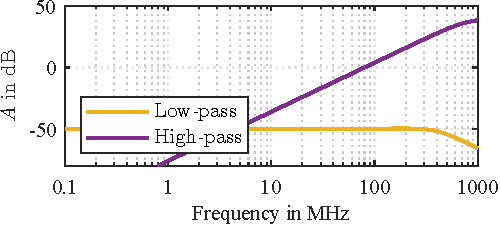
\includegraphics[scale = 1]{figures/3_Methods/Highpass/TF_FD.pdf}
		\caption{Transfer function of conventional low-pass measurement and second order high-pass.}
	\end{subfigure}%
	\hfill
	\begin{subfigure}{0.48\textwidth}
		\centering
		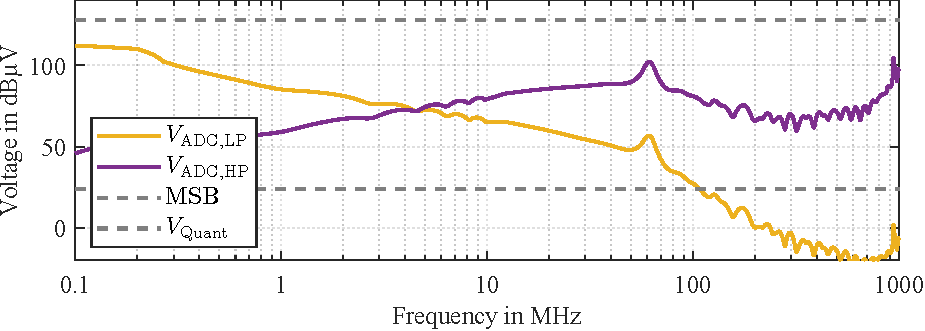
\includegraphics[scale = 1]{figures/3_Methods/Highpass/ADC_sig.pdf}
		\caption{Effective voltage spectrum of low-pass and high-pass measurements at the oscilloscope input with the respective quantization-noise floor.}
	\end{subfigure}
	\caption{Measurement principle of a high-pass measurement for EMC-relevant frequency components of a transient signal.}\label{fig:QuantNoise_wHP}
\end{figure}

To compensate for the transfer function and reconstruct the original signal, the high-pass probe is modeled as a linear time-invariant (LTI) system with impulse response $\mi{a}{HP}(t)$ and frequency-domain transfer function $\mi{A}{HP}(f)$.
At the oscilloscope input, the measured signal is the convolution of the drain-source voltage with the probe response:
\begin{equation}
	\mi{v}{DS,HP,raw}(t) = \mi{a}{HP}(t) \ast \mi{v}{DS}(t),
\end{equation}

which in the frequency domain becomes a multiplication:
\begin{equation}
	\mi{V}{DS,HP,raw}(f) = \mi{A}{HP}(f) \cdot \mi{V}{DS}(f).
\end{equation}

To recover the original drain-source voltage spectrum, the measured signal is compensated by the transfer function:
\begin{equation}
	\mi{V}{DS,HP,comp}(f) = \frac{\mathcal{F}\{\mi{v}{DS,HP,raw}(t)\}}{\mi{A}{HP}(f)} = \frac{\mi{V}{DS,HP,raw}(f)}{\mi{A}{HP}(f)}.
	\label{eq:HP_comp}
\end{equation}

In logarithmic representation, this division becomes a simple subtraction of the probe gain curve $\mi{A}{HP}(f)$:
\begin{equation}
	\mi{V}{DS,HP,comp}^{\text{dB}\upmu\text{V}} = \mi{V}{DS,HP,raw}^{\text{dB}\upmu\text{V}} - \mi{A}{HP}^{\text{dB}}.
\end{equation}

As a result, the measurement is no longer limited by the onset of the noise floor, but primarily by the bandwidth of the probe and additional noise introduced by the high-pass filter.

